% =====================================================================
%  Основное содержимое отчёта.
% =====================================================================

\labpart{Структура разработанной системы}

Реферирование документов реализовано как новый сценарий использования
поверх архитектуры ЛР1--ЛР2 (см. \texttt{docs/ARCHITECTURE.md}):
границы сервисов по-прежнему проведены по зоне ответственности, а не по
лабораторной работе, поэтому ЛР3 добавляет один новый сервис и новые
таблицы БД, не меняя ни одного существующего контракта системы.
Структура системы на уровне контейнеров (C4, уровень 2) показана на
рисунке~\ref{fig:architecture-c4}; компоненты и связи, добавленные
именно в этой лабораторной работе, выделены зелёным цветом.

\pumldiagram{architecture-c4}{Диаграмма контейнеров разработанной системы (нотация C4); зелёным -- новое в ЛР3}{architecture-c4}{0.95}

Новый сервис \texttt{summarization-service} (Python, FastAPI +
\texttt{nlp\_core}) -- углублённый элемент варианта 16 (реализация
методов реферирования). Он, как и \texttt{nlp-service} и
\texttt{lang-id-service}, не хранит состояние и не обращается к БД
самостоятельно: получает на вход уже подготовленные данные (текст,
веса терминов документа, эмбеддинги предложений) и возвращает чистый
результат вычисления -- отобранные предложения с их весами либо
иерархический список ключевых слов. Оркестрацией (какие документы
проиндексированы, что сохранить в БД, что показать пользователю)
занимается \texttt{api}, как и для остальных сценариев системы. Веса
терминов документа (модифицированный TF-IDF) для алгоритмического
метода считаются в \texttt{api} тем же кодом, что и для ключевых слов
-- переиспользуется формула ЛР1 \texttt{modified\_term\_weight}. Помимо
нового сервиса, ЛР3 расширила ответственность \texttt{frontend}:
\begin{itemize}
  \item новая страница «Реферирование» с двумя вкладками (реферат
  документа, тестирование на коллекции);
  \item поиск документа реализован не выпадающим списком со всеми
  документами коллекции, а комбобоксом с поиском на сервере
  (\texttt{DocumentCombobox}) -- по мере набора текста подгружается
  только страница из не более чем 30 совпадающих по названию
  документов (аналогично добавлен параметр \texttt{search} в
  \texttt{GET /collections/\{id\}/documents}, реализованный через
  \texttt{ILIKE} с экранированием служебных символов LIKE). Так список
  остаётся быстрым и при выборе из коллекции на 20 документов, и из
  коллекции на несколько тысяч -- в отличие от предыдущего варианта,
  подгружавшего до 500 документов целиком в один выпадающий список;
  \item кнопка «Печать» открывает не системную печать всей страницы
  приложения, а отдельную вкладку с Blob URL, содержащую только текст
  реферата, иерархию ключевых слов и (если оно было построено)
  перефразированную LLM версию -- без интерфейса приложения;
  результат сохраняется в файл в том же составе.
\end{itemize}

\labpartbreak{Структура базы данных}

Схема ключевых таблиц и связей между ними показана на
рисунке~\ref{fig:database-erd} (нотация Crow's Foot); таблицы,
добавленные в ЛР3, выделены зелёным.

\pumldiagram{database-erd}{ER-диаграмма базы данных (нотация Crow's Foot); зелёным -- новое в ЛР3}{database-erd}{1.0}

Структуры данных для входной и выходной информации методов
реферирования:
\begin{itemize}
  \item \textbf{вход} -- \texttt{documents.clean\_text} (тот же
  очищенный текст документа, что используется для индексации в ЛР1) и
  веса терминов документа, вычисляемые по требованию (не кешируются
  отдельной таблицей, т.к. пересчёт дешевле хранения ещё одной копии
  весов рядом с уже существующей \texttt{term\_weights});
  \item \textbf{выход (результат одного реферата)} --
  \texttt{document\_summaries}: метод, отобранные предложения
  (\texttt{summary\_sentence\_indices}), общее число предложений
  документа, затраченное время и \texttt{total\_chars} -- длина
  документа в символах, добавленная в ЛР3 специально для корректного
  расчёта степени сжатия (см. далее);
  \item \textbf{выход (результат тестового прогона)} --
  \texttt{summarization\_runs} (одно тестирование одного метода на
  всех документах коллекции, статус и прогресс для живого
  прогресс-бара, по аналогии с \texttt{lang\_id\_runs} из ЛР2) и та же
  \texttt{document\_summaries} (поле \texttt{run\_id} отличает разовый
  реферат от строки, принадлежащей тестовому прогону);
  \item \textbf{выход (перефразирование)} --
  \texttt{document\_summary\_polishes}: текст после обработки LLM и
  использованная модель, отдельная таблица (а не поле у
  \texttt{document\_summaries}), т.к. один реферат можно
  перефразировать повторно.
\end{itemize}

\labpart{Основные алгоритмы}

Общая схема построения реферата одного документа показана на
рисунке~\ref{fig:summarization-pipeline}; методы отличаются только
правилом расчёта веса предложения (шаг 2), реферат-список ключевых
слов (шаг 4) строится один раз и не зависит от метода отбора
предложений.

\pumldiagram{summarization-pipeline}{Построение реферата одного документа (общая схема для всех трёх методов)}{summarization-pipeline}{0.85}

\textbf{Алгоритм из методички.} Вес предложения -- произведение трёх
функций:
\begin{equation}
  \text{Вес}(S_i) = \mathrm{Posd}(S_i) \cdot \mathrm{Posp}(S_i) \cdot \mathrm{Score}(S_i),
\end{equation}
где $\mathrm{Posd}(S_i) = 1 - BD(S_i)/|D|$ и $\mathrm{Posp}(S_i) = 1 -
BP(S_i)/|P|$ -- положение предложения в документе и в абзаце
(предложения ближе к началу весят больше), а $\mathrm{Score}(S_i) =
\sum_{t \in S_i} tf(t, S_i) \cdot w(t, D)$ -- сумма модифицированного
TF-IDF веса терминов предложения (та же формула $w(t,D) = 0{,}5 \cdot
(1 + tf/tf_{\max}) \cdot \log(|DB|/df(t))$, что и в ЛР1).

\textbf{TextRank.} Графовый метод: предложения -- вершины, вес ребра
между $S_i$ и $S_j$ -- пересечение множества лемм, нормированное по
длине предложений:
\begin{equation}
  w_{ij} = \frac{|W_i \cap W_j|}{\log(|W_i|+1) + \log(|W_j|+1)},
\end{equation}
итоговый вес предложения -- результат PageRank по этому графу
(damping~$=0{,}85$, до сходимости или 100 итераций). Не требует
индексации коллекции и работает по каждому документу независимо.

\textbf{Эмбеддинги.} Каждое предложение кодируется моделью OpenRouter
(та же модель, что и для семантического поиска в ЛР1); вес предложения
-- косинусная близость его эмбеддинга к центроиду эмбеддингов всех
предложений документа. Для всех трёх методов итоговый реферат --
$N$ предложений с наибольшим весом, возвращённые к исходному порядку
следования в документе.

\textbf{Реферат-список ключевых слов.} Корневые термины -- весь
словарь документа (все термины с ненулевым модифицированным TF-IDF
весом), отсортированный по убыванию веса, без искусственного
ограничения сверху (общий для всех трёх методов расчёт, не зависит от
способа отбора предложений) -- для коротких тестовых текстов это
означает, что дерево ключевых слов покрывает всю лексику документа, а
не только первые 15 самых весомых терминов, как было в первой версии
реализации. Словосочетания-дети строятся без синтаксического
парсера: последовательные прилагательные/существительные текста
(POS-теги spaCy) длиной $\geq 2$ слов -- кандидаты в словосочетания,
каждое оценивается суммой весов входящих в него терминов и
закрепляется за тем корнем с наибольшим весом среди уже
незанятых корней, который оно содержит (не более 5 словосочетаний на
корень). Корень без подходящих словосочетаний остаётся листом дерева
-- так реферат остаётся корректным и для документов, где нет
устойчивых словосочетаний вокруг темы. Пример результата -- на
рисунке~\ref{fig:keyword-hierarchy}.

\begin{figure}[H]
  \centering
  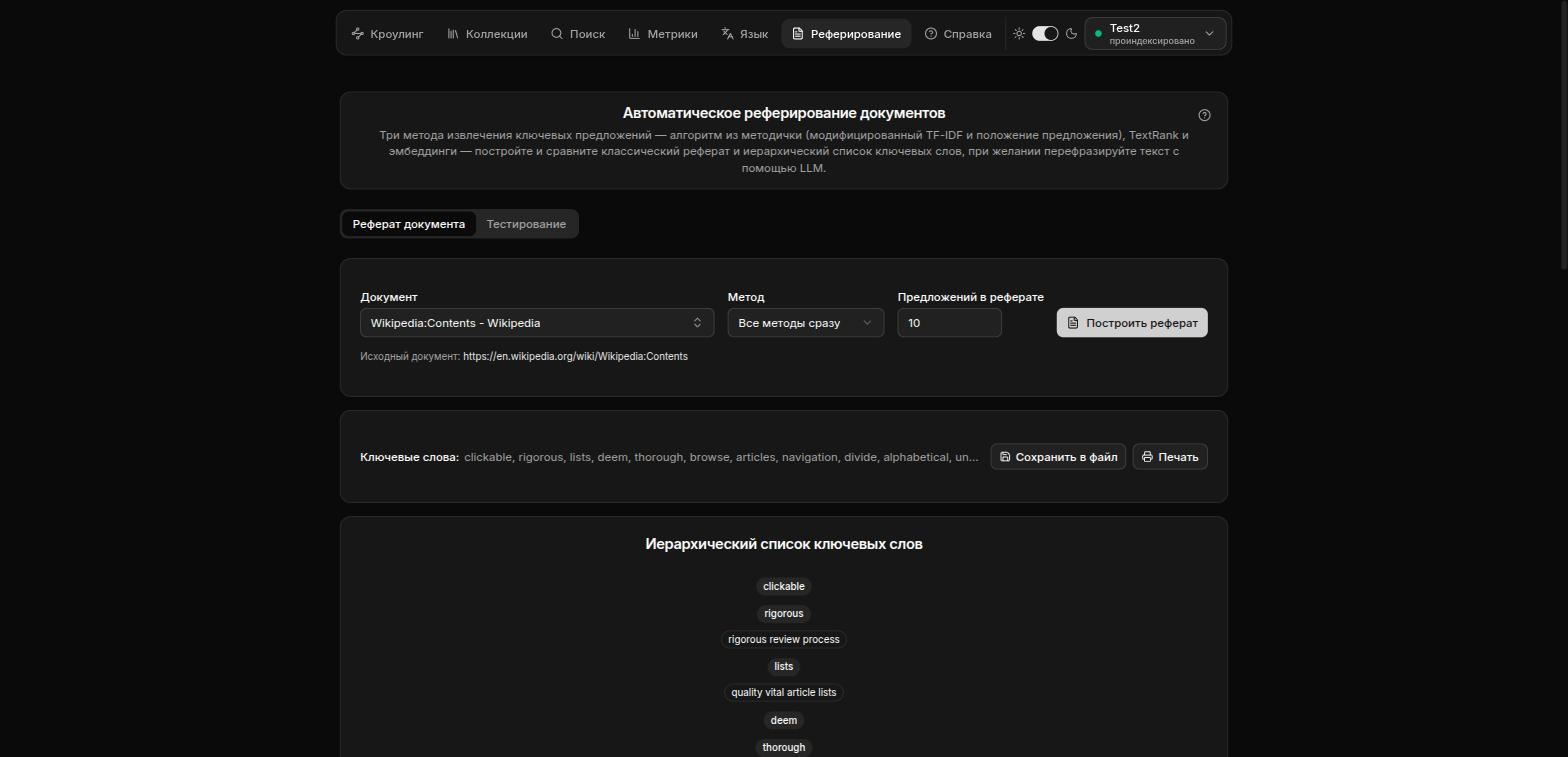
\includegraphics[width=0.85\textwidth]{lab/pictures/keyword_hierarchy.png}
  \caption{Вкладка «Реферат документа»: реферат-список ключевых слов в виде дерева (корень -- словосочетания, в которые он входит)}
  \label{fig:keyword-hierarchy}
\end{figure}

При выборе метода «Все методы сразу» рефераты всех трёх методов
строятся одним запросом и выводятся друг под другом (не в колонках) --
рисунок~\ref{fig:methods-vertical}; перефразированная LLM версия
реферата появляется прямо под тем методом, к которому она относится
(рисунок~\ref{fig:llm-paraphrase}).

\begin{figure}[H]
  \centering
  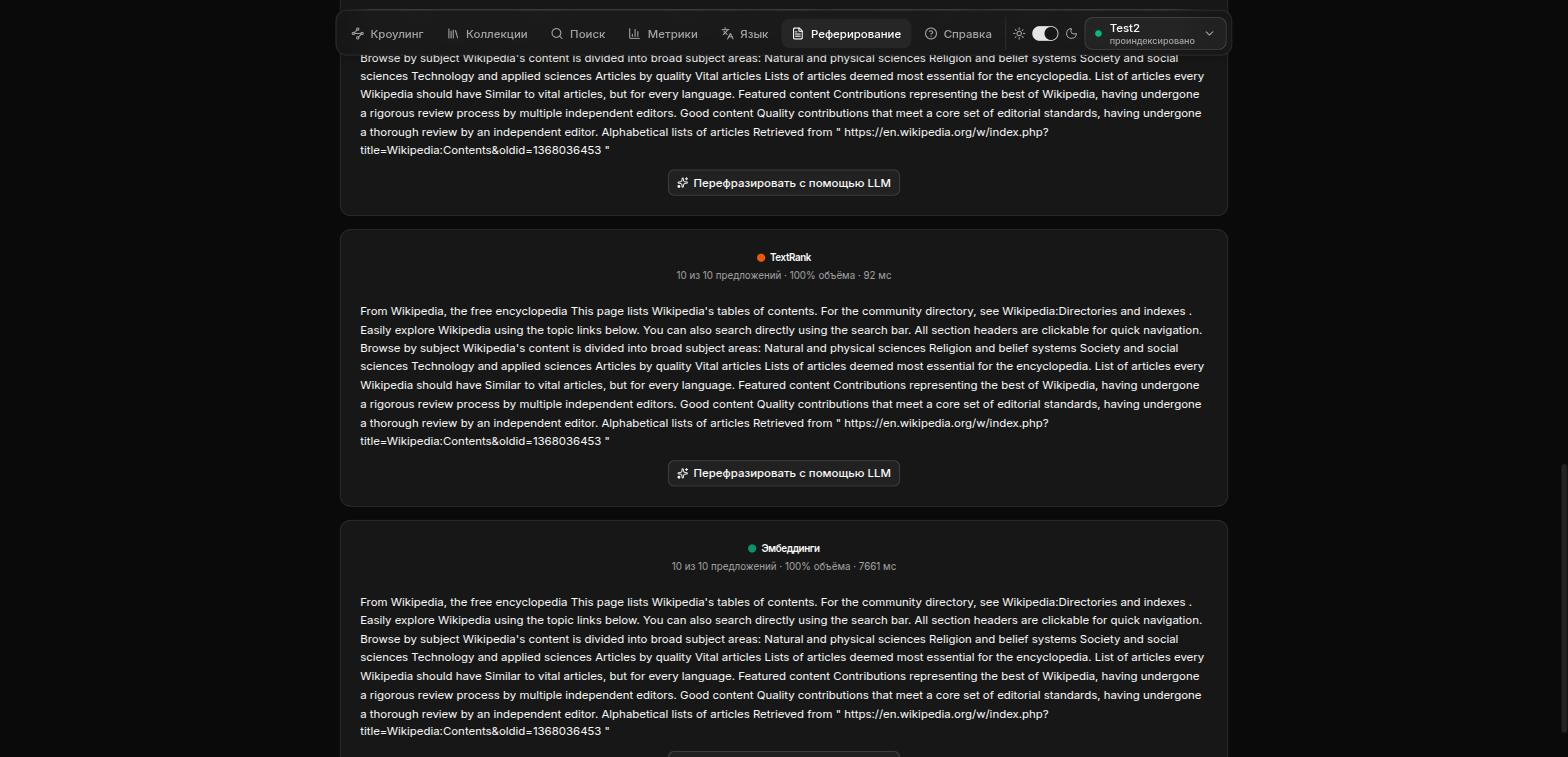
\includegraphics[width=0.85\textwidth]{lab/pictures/methods_vertical.png}
  \caption{Результаты всех трёх методов, построенные одним запросом («Все методы сразу») и выведенные друг под другом}
  \label{fig:methods-vertical}
\end{figure}

\begin{figure}[H]
  \centering
  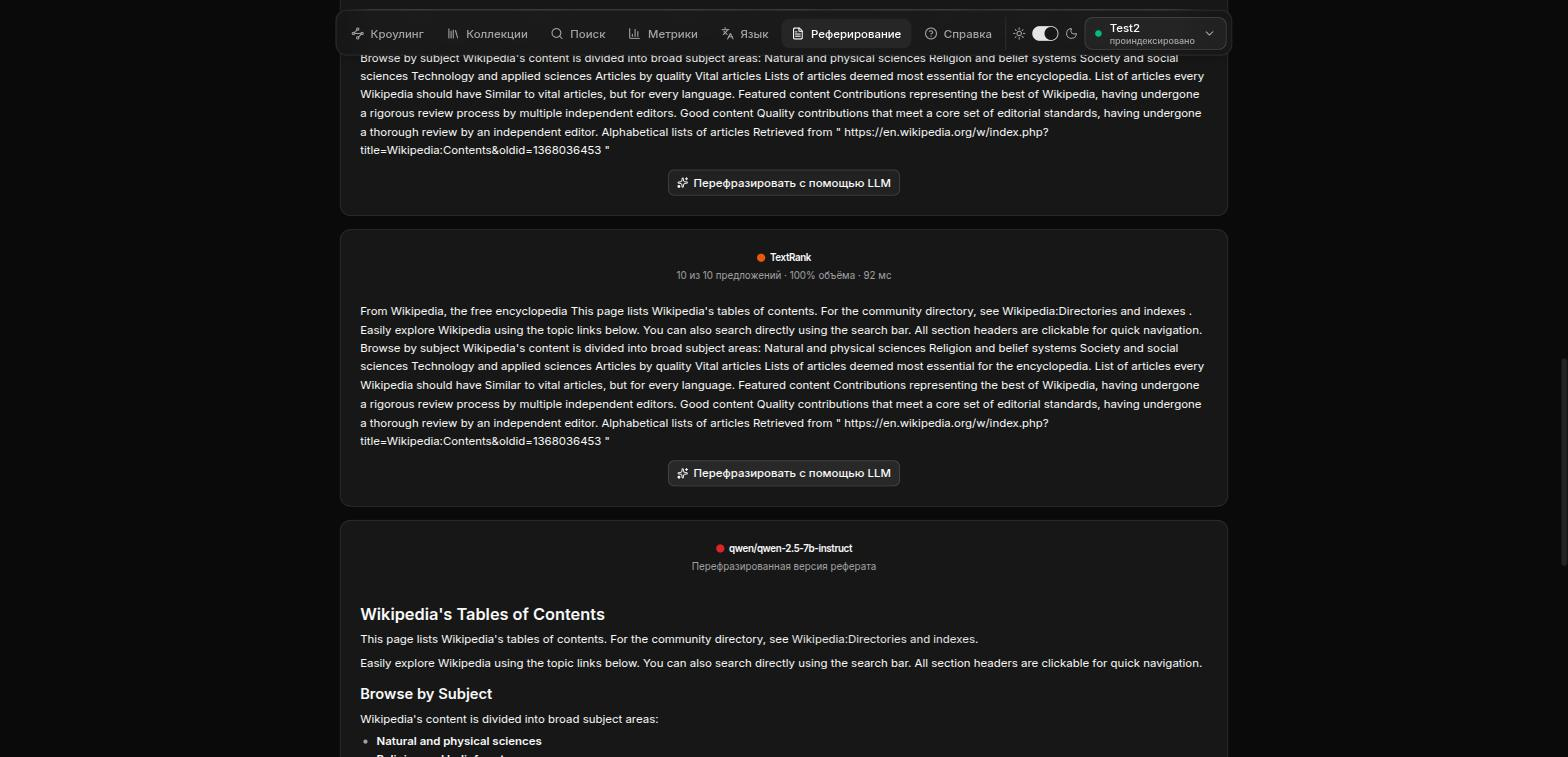
\includegraphics[width=0.85\textwidth]{lab/pictures/llm_paraphrase.png}
  \caption{Перефразированная с помощью LLM версия реферата под соответствующим методом}
  \label{fig:llm-paraphrase}
\end{figure}

\textbf{Перефразирование через LLM.} Запрос к модели состоит из
системного промпта (листинг~\ref{lst:llm-system-prompt}, задаёт
единственную задачу -- лёгкую правку уже отобранных предложений без
добавления, удаления или дальнейшего сокращения информации) и
пользовательского сообщения, равного тексту реферата (с необязательной
пометкой языка первой строкой, если он известен из карточки документа).
Такой узкий промпт -- единственная защита от типичной проблемы LLM в
задаче реферирования: модель дописывает отсутствующие в источнике факты
или самостоятельно сокращает текст ещё раз, из-за чего результат
перестаёт быть точным отражением уже отобранных алгоритмом предложений.

\begin{codelisting}{text}{Системный промпт для LLM-полировки реферата (\texttt{services/nlp-service/app/llm.py})}{llm-system-prompt}
You are a copy-editing assistant for an extractive text-summarization tool. You are given sentences that an algorithm already selected as the most important ones from a source document. Your ONLY task is to lightly polish them into a clean, coherent passage: fix grammar, smooth the transitions between sentences, and resolve obviously dangling pronouns/references when the antecedent is already present in the given text.

Strict rules:
1. Do NOT add any fact, number, claim, or detail that is not already present in the input sentences.
2. Do NOT omit or change the meaning of any of the given sentences.
3. Do NOT summarize further -- keep all the given information.
4. Write in the same language as the input text.
5. Respond in Markdown: plain paragraphs are enough, only use headings, lists or emphasis if they genuinely improve readability of this exact content.
\end{codelisting}

\labpartbreak{Тестовая коллекция документов}

Тестовая коллекция -- та же коллекция англоязычных статей Wikipedia,
наполненная краулером ЛР1 (глубина 3, переход только в пределах
домена \texttt{en.wikipedia.org}), что используется для проверки
поиска: 20 проиндексированных документов, на которых алгоритмический
метод может рассчитать модифицированный TF-IDF (без индексации
коллекции доступны только TextRank и метод на эмбеддингах, не
требующие весов терминов). Число предложений в реферате -- 10 (по
умолчанию, как рекомендует методичка); фактическое среднее число
отобранных предложений -- 7{,}3, т.к. часть документов короче 10
предложений и для них отбираются все доступные.

\labpart{Результаты тестирования и оценка качества}

Каждый из трёх методов протестирован на всех 20 документах коллекции;
средние по документам метрики приведены в таблице~\ref{tab:metrics-summarization},
тот же расчёт в интерфейсе системы -- на рисунке~\ref{fig:methods-comparison}
(вкладка «Тестирование»).

\begin{table}[H]
  \centering
  \caption{Метрики качества и быстродействия по 20 документам тестовой коллекции}
  \label{tab:metrics-summarization}
  \begin{tabularx}{\textwidth}{|X|r|r|r|}
    \hline
    Метрика & Алгоритм из методички & TextRank & Эмбеддинги \\
    \hline
    Среднее время реферирования & 534{,}26 мс & 289{,}45 мс & 4013{,}54 мс \\
    \hline
    Средняя степень сжатия & 70{,}4\,\% & 69{,}6\,\% & 65{,}9\,\% \\
    \hline
    Среднее число предложений в реферате & 7{,}3 & 7{,}3 & 7{,}3 \\
    \hline
    Документов обработано & 20 & 20 & 20 \\
    \hline
  \end{tabularx}
\end{table}

\begin{figure}[H]
  \centering
  
\includegraphics[width=\textwidth]{lab/pictures/methods_comparison.png}
  \caption{Вкладка «Тестирование»: сравнение методов по времени и степени сжатия, результаты по документам с экспортом (CSV/JSON) и печатью}
  \label{fig:methods-comparison}
\end{figure}

\textbf{Степень сжатия считается по длине текста в символах, а не по
числу предложений.} Изначально степень сжатия считалась как отношение
числа отобранных предложений к общему числу предложений документа. Все
три метода при сравнении на одной коллекции получают на вход один и
тот же \texttt{sentence\_count} и работают с одним и тем же
документом (тем же числом предложений), поэтому такое отношение
математически гарантированно совпадает у всех трёх методов -- оно
вообще не зависит от того, какие именно предложения выбрал метод, а
только от того, сколько предложений было запрошено. Как метрика
сравнения методов она была бесполезна по построению, а не только
случайно совпадала на конкретных данных. Метрику пересчитали на длину
извлечённого текста в символах относительно длины документа
(\texttt{total\_chars}, таблица~\ref{tab:metrics-summarization}) --
эта величина действительно зависит от того, какие (более короткие или
более длинные) предложения выбрал метод, и поэтому различает методы
(70{,}4~/~69{,}6~/~65{,}9\,\%, таблица~\ref{tab:metrics-summarization}).

\labpart{Анализ результатов и предложения по улучшению}

\begin{enumerate}
  \item \textbf{TextRank -- самый быстрый метод, эмбеддинги -- самый
  медленный, разница на порядок.} Среднее время на документ --
  289{,}45~мс у TextRank против 534{,}26~мс у алгоритма из методички и
  4013{,}54~мс у метода на эмбеддингах (табл.~\ref{tab:metrics-summarization}).
  TextRank работает целиком локально (лемматизация и граф
  предложений); алгоритмический метод дополнительно обращается к БД за
  весами терминов; метод на эмбеддингах ждёт HTTP-round-trip к
  OpenRouter на каждое предложение документа -- сетевая задержка
  доминирует над самим вычислением косинусной близости.
  \item \textbf{Алгоритм из методички даёт самую высокую степень
  сжатия, эмбеддинги -- самую низкую (70{,}4 против 65{,}9\,\%).}
  Правдоподобное объяснение, вытекающее из самого правила отбора:
  $\mathrm{Posd}$ отдаёт предпочтение предложениям в начале документа,
  а первые предложения статей Wikipedia (как правило, развёрнутое
  вводное предложение-определение) в среднем длиннее рядовых; метод на
  эмбеддингах ищет предложение, ближайшее к семантическому центроиду
  документа, а такие предложения чаще короче и конкретнее (единичный
  факт, а не общее вводное описание). TextRank -- посередине, так как
  граф пересечения лемм не даёт систематического смещения ни к началу
  документа, ни к длине предложения.
  \item \textbf{Что можно добавить в систему для её улучшения.}
  \begin{itemize}
    \item ограничение реферата по символам/словам, а не только по
    числу предложений -- при сильно отличающейся длине предложений
    между документами текущий параметр (число предложений) даёт менее
    предсказуемый по факту итоговый объём текста, чем прямое
    ограничение длины;
    \item кеширование весов терминов документа (сейчас пересчитываются
    заново при каждом построении реферата и при каждом документе
    тестового прогона) -- ускорило бы прежде всего алгоритмический
    метод при повторных запусках на одной коллекции;
    \item синтаксический парсер (dependency parsing) вместо текущего
    эвристического выделения словосочетаний по последовательным
    ADJ/NOUN-тегам -- корректно бы разделял, например, однородные
    члены и не склеивал случайно соседние по тексту, но синтаксически
    не связанные слова в одно словосочетание;
    \item параллельные запросы эмбеддингов предложений вместо
    последовательных -- основная причина отставания метода на
    эмбеддингах по скорости, ограничение сейчас только на стороне
    клиента nlp-service.
  \end{itemize}
  \item \textbf{Где систему можно применить.}
  \begin{itemize}
    \item построение краткой выжимки и облака тем для документов,
    найденных информационно-поисковой системой ЛР1 -- перед открытием
    полного текста;
    \item предварительный просмотр содержимого перед разметкой
    истинного языка/релевантности в ЛР1--ЛР2 -- реферат и ключевые
    слова быстрее прочитать, чем весь документ;
    \item учебный полигон для последующих лабораторных работ курса,
    использующих понятие значимого предложения/термина документа
    (например, генерация ответов на естественно-языковые запросы) --
    веса терминов и разбиение на предложения уже переиспользуются из
    ЛР1 и общей библиотеки \texttt{nlp\_core}.
  \end{itemize}
\end{enumerate}

\labpartbreak{Использованные готовые компоненты}

\begin{table}[H]
  \centering
  \caption{Библиотеки и программные средства, использованные при реализации ЛР3 (дополнительно к перечисленным в отчётах по ЛР1--ЛР2)}
  \label{tab:stack-summarization}
  \small
  \begin{tabularx}{\textwidth}{|l|X|}
    \hline
    Компонент & Назначение \\
    \hline
    spaCy (POS-теги, \texttt{tok.pos\_}) & Выделение кандидатов в
      словосочетания для реферата-списка ключевых слов -- те же
      теги, что уже использовались для лемматизации в ЛР1, без
      дополнительных моделей. \\
    \hline
    qwen/qwen-2.5-7b-instruct (через OpenRouter) & Перефразирование
      уже отобранных предложений -- небольшая и дешёвая модель со
      строгим промптом (только грамматика и связность, без новых
      фактов), та же интеграция OpenRouter, что и для эмбеддингов. \\
    \hline
    Qwen3-Embedding-8B (через OpenRouter) & Источник эмбеддингов
      предложений для метода на эмбеддингах -- та же модель, что и в
      ЛР1/ЛР2; для реферата отдельного документа эмбеддинги считаются
      по предложениям (не по документу целиком, как в ЛР1). \\
    \hline
  \end{tabularx}
\end{table}
